\section{Reynolds effects}
We are now interested to catch the effects of the Reynolds on our statistics.\\~\par
The firstly macroscopical effect that we face is a shift, towards higher values, of the mean velocity profile. The shadowed area of figure~\ref{mean:comparison} let us enjoy the previous statement. According to this graph we can see a progressive narrowing of the region subjected to the higher shear stress, as the Reynolds number becomes larger.\par
Under the previous graph we reported the same quantity, but presented in semi-logaritmic scale, using both inner and outer scaling.
The first plot of figure~\ref{loglaw:comparison} highlights the results of the simulations and the theoretical behavior expectations.
In particular we can see that, despite the Reynolds number, all the simulations present the linear $\bar{u}=y^{+}$ behavior expected in the viscous sublayer, and the logarithmic profile in the homonym region, with $k=0.41$ and $B=5.2$.\\~\par

\begin{figure}
\begin{center}
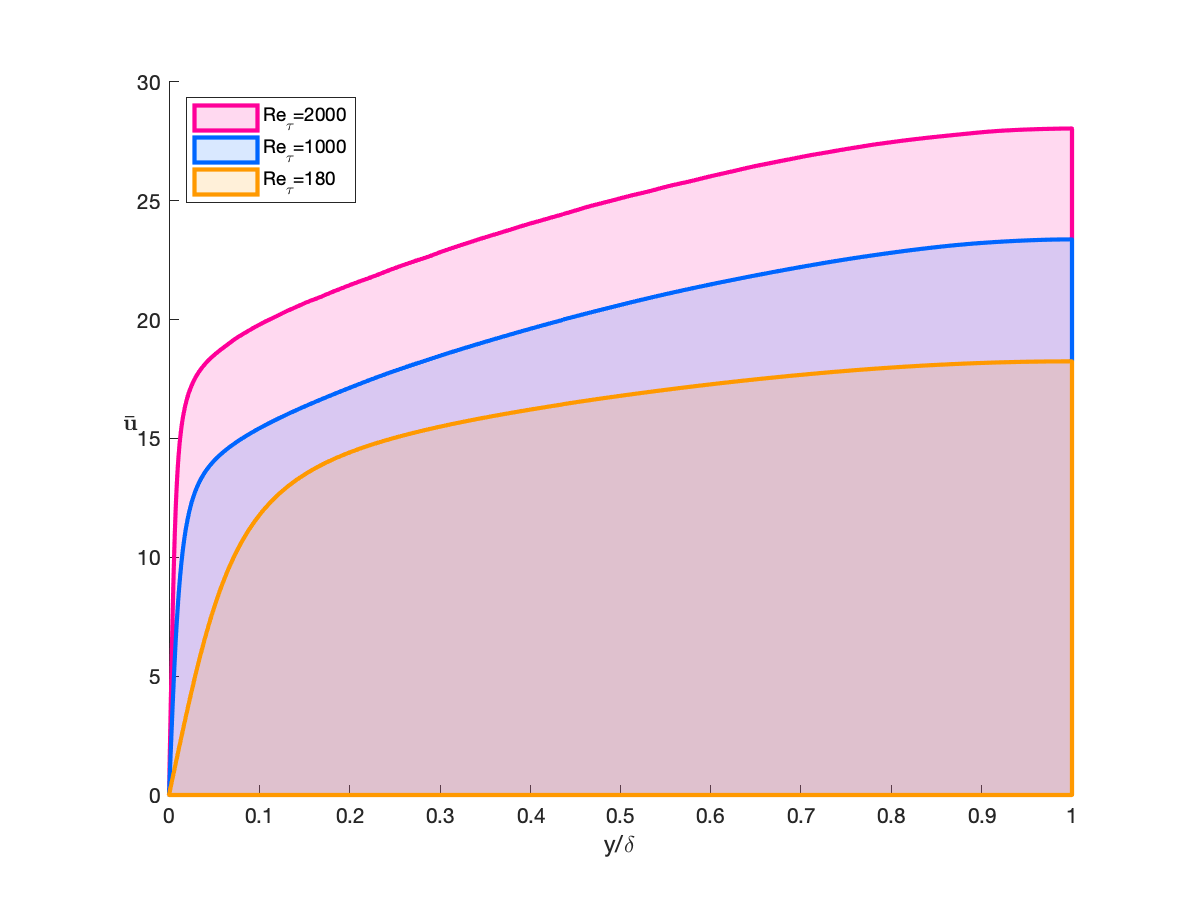
\includegraphics[scale=0.55]{grafici/u_mean_comparison.eps}
\caption{Mean velocity profile at $Re_{\tau}$ variation}
\label{mean:comparison}
\end{center}
\end{figure}
\begin{figure}
\begin{center}
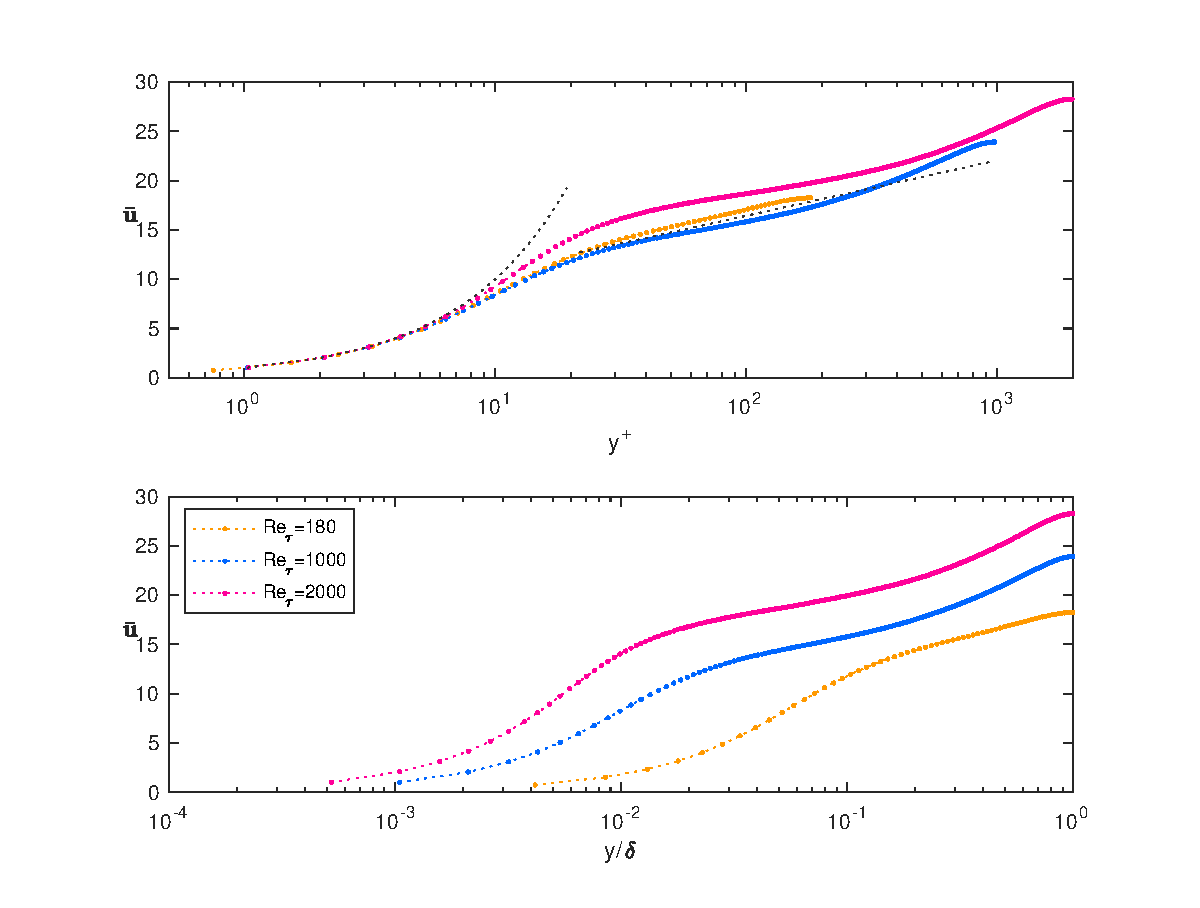
\includegraphics[scale=0.55]{grafici/loglaw_comparison.eps}
\caption{The law of the wall, in inner and outer scaling, at $Re_{\tau}$ variation}
\label{loglaw:comparison}
\end{center}
\end{figure}


Differently, the Reynolds stresses and the viscous stress exhibit dependance on the Reynolds number.\par
Figure~\ref{shear:comparison} shows how the shear stress components modify as the Reynolds number increase. \par
Focusing on the normalized Reynolds stresses graph we can clearly see that, as the $Re_{\tau}$ increase, the region subjected to this kind of stresses becomes larger, with the peak moving towards the wall. Such kind of stress is associated with the fluid turbulent motions, therefore it was expectable a raise of this components as we move towards a more turbulent flow. \par

\begin{figure}
\begin{center}
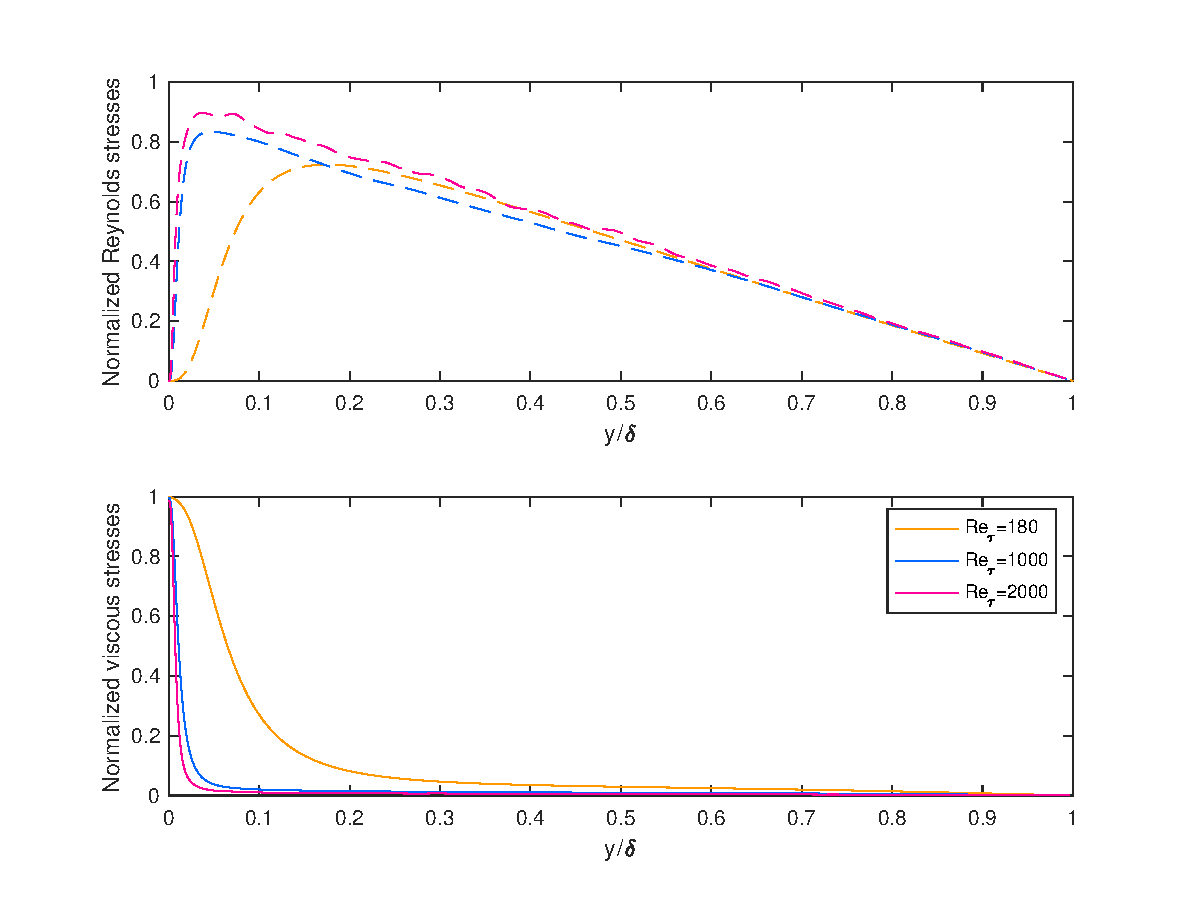
\includegraphics[scale=0.55]{grafici/shear_comparison.eps}
\caption{Normalized shear profiles at $Re_{\tau}$ variation}
\label{shear:comparison}
\end{center}
\end{figure}

\begin{figure}
\begin{center}
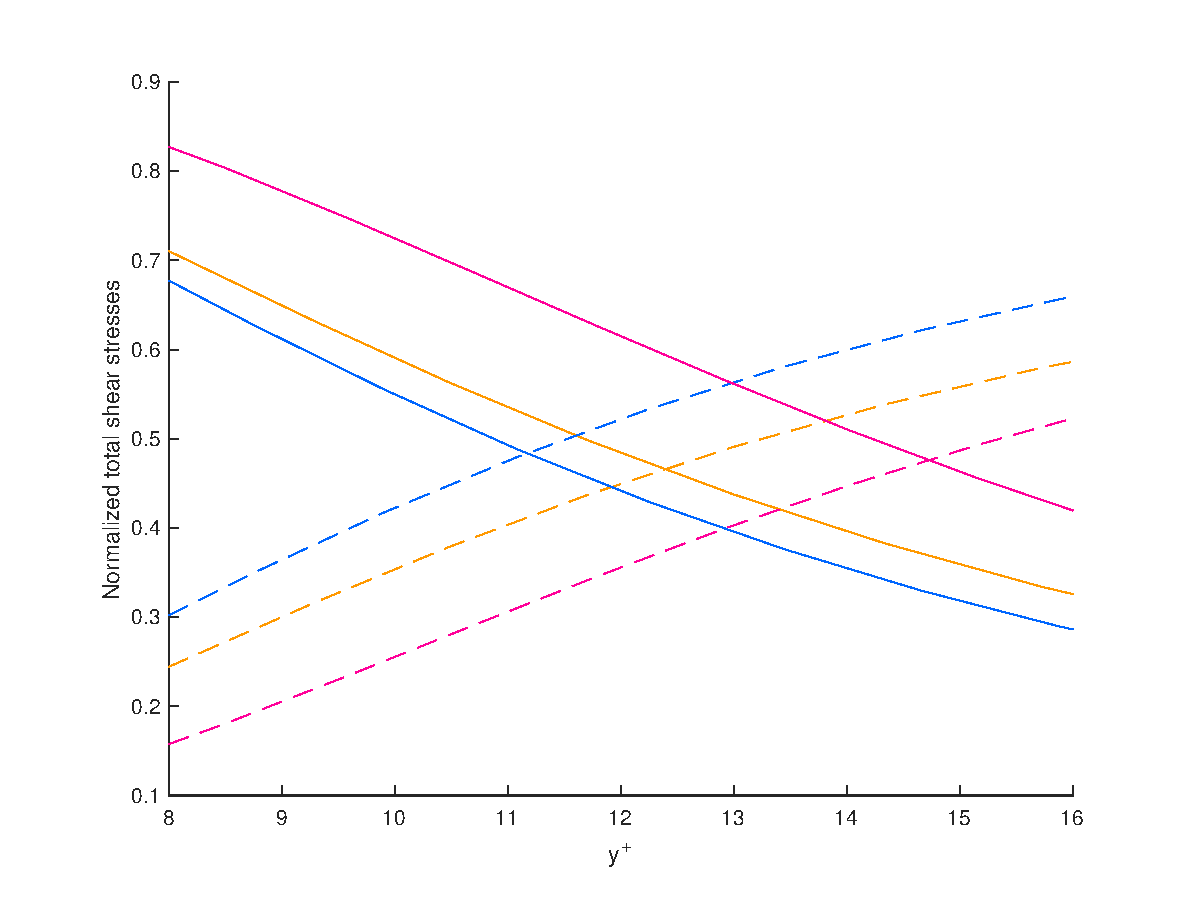
\includegraphics[scale=0.55]{grafici/y12.eps}
\caption{Particular of the shear stress, at $Re_{\tau}$ variation}
\label{y12}
\end{center}
\end{figure}

On the other side the contribute of the viscous stress, associate to $\partial{\bar{u}}/\partial{t}$, is maximum at the wall and tends to become negligible as we move towards the centerline. \par
As testified by figure~\ref{loglaw:comparison}, the higher is the Reynolds and the wider is the area subjected to logarithmic profile, hence smaller is the area subjected to strong variation of the mean velocity profile with the wall-normal coordinate. This fact reflects on our shear component reducing its range of effectiveness to few units, close to the wall, as the $Re$ grows.\par
Although, in terms of outer scaling, the stress components are subjected to strong variations, in inner scaling we can see, in figure~\ref{y12}, that the point at which the two components cross themself remains quite constant, with an $y^{+}$ around 12 wall-units.\\~\par


\begin{figure}
\begin{center}
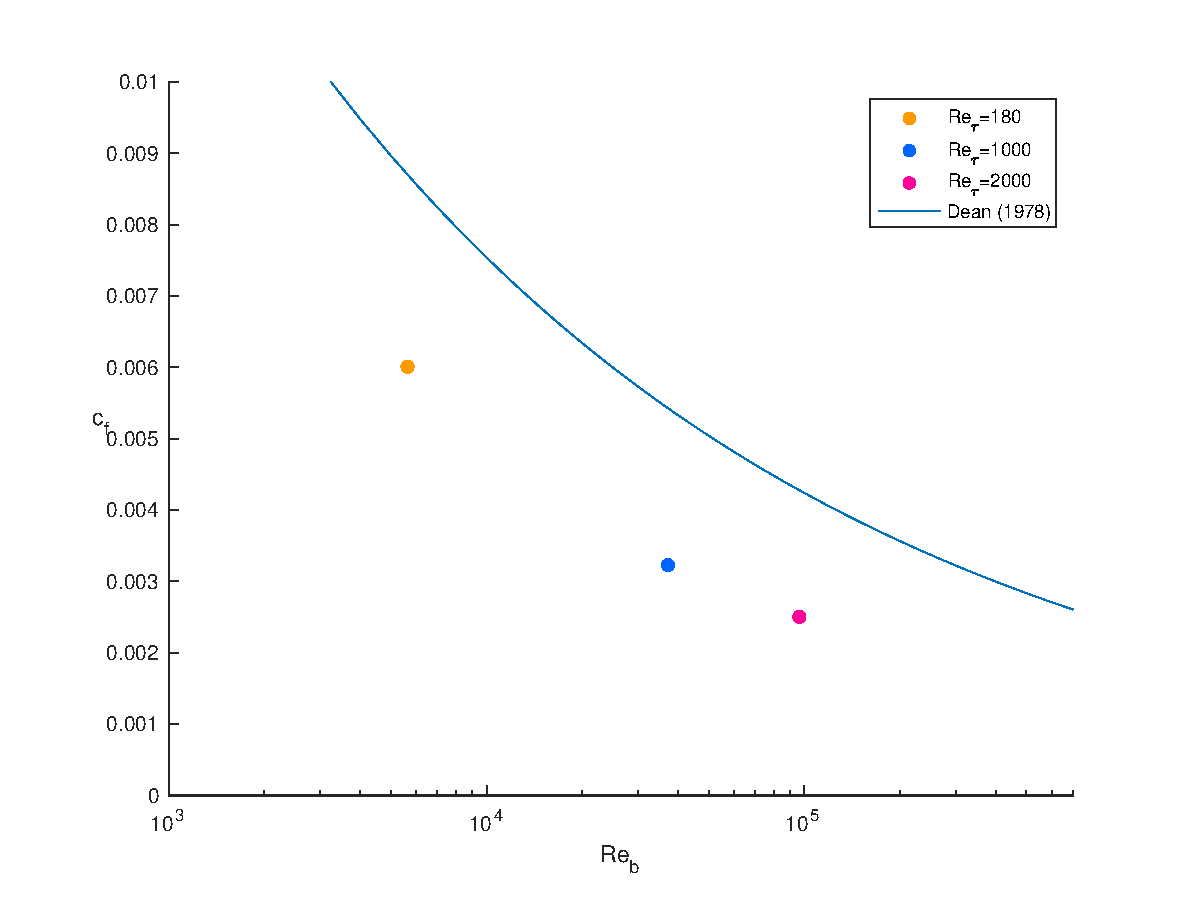
\includegraphics[scale=0.55]{grafici/cf.eps}
\caption{Dependance of the $c_{f}$ from $Re_{b}$}
\label{cf}
\end{center}
\end{figure}


One of the most important flow property for wall bounded flows is the friction coefficient.
The $c_{f}$ has been studied in detail by many famous authors of the past: Nikuradse, Prandtl, Blasius just to cite some of them. \par
In our simulations we computed the skin friction coefficient based on the definition provided by~\cite[279]{pope}, based on centerline velocity $(U_{0})$ and the $Re_{b}$ of the channel.
The quantities have been defined as
\begin{equation*}
c_{f}= 2(\frac{u_{\tau}}{U_{0}})^{2}	\quad~\quad~\quad~\quad	Re_{b}= \frac{2 U_{b} \delta}{\nu},
\end{equation*}
and the results have been reported on figure~\ref{cf}. \par
Our $c_{f}$ shows good fitting with the results of the experimental campaign of Dean reported in~\cite{Dean}.


